\chapter{基于Kagome晶格的声学哈密顿量推导及边界条件对拓扑态的影响研究}

\section{引言}

\section{Kagome晶格与声学结构类比}

\begin{figure}[h!]
  \centering
  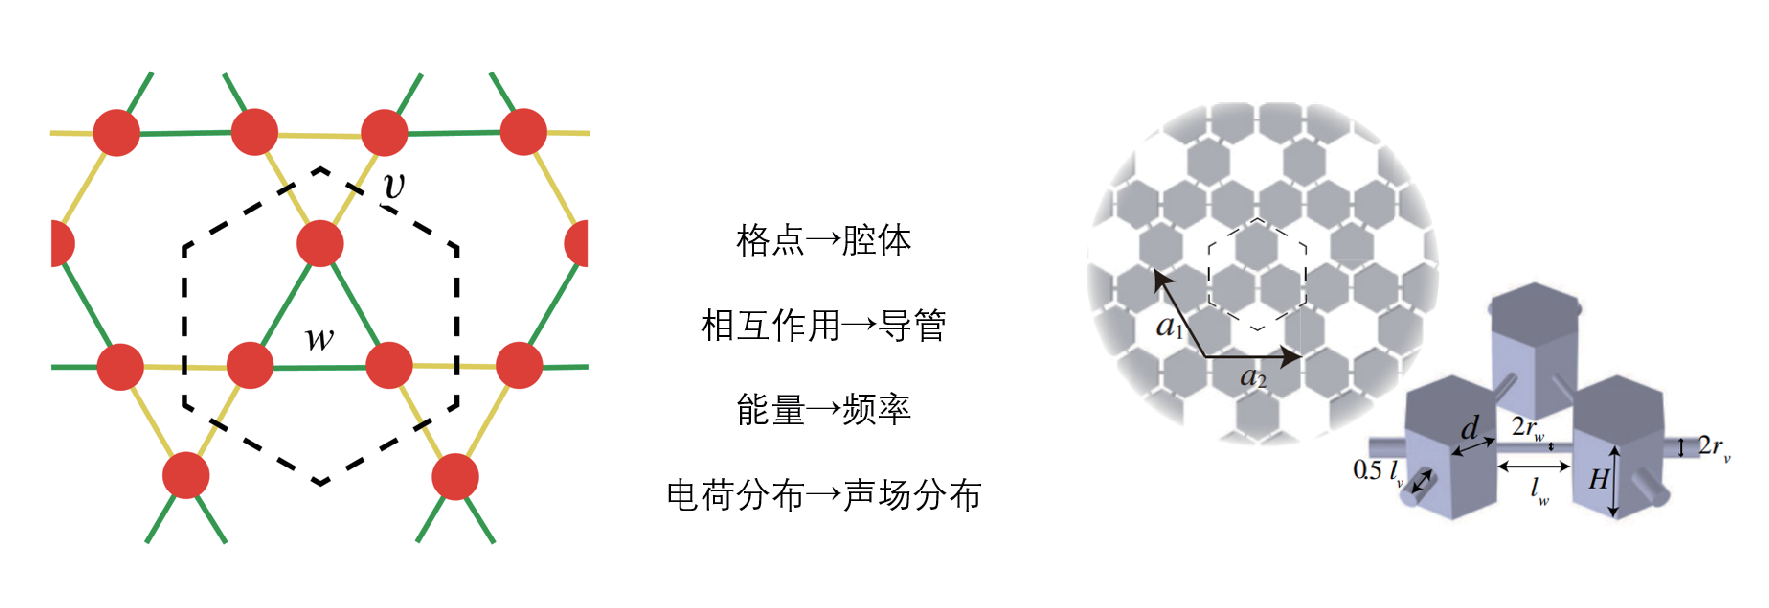
\includegraphics[width=1\textwidth]{images/fig3-1.eps} 
  \caption{以Kagome结构为例,电子系统与声学系统存在显著的相似性。}
  \label{fig_3_1}
\end{figure}

在物理学中,电子系统与声学系统存在显著的相似性。电子系统里,格点、相互作用、能量、电荷分布是关键要素;而在声学系统中,可类比为腔体、导管、频率、声场分布。以图\ref{fig_3_1}的Kagome晶格为例,以下是电子系统和声学系统中几个要素的相似性详细解释:
\begin{itemize}
  \item 格点与腔体:在电子系统的晶格模型中,格点是电子所处的位置,电子在这些格点上具有一定的能量状态和量子特性。格点的排列和相互关系决定了电子的能带结构等重要物理性质。而在声学系统中,我们可以把单个腔体看作是一个共振单元,它也具有共振频率和对应的共振模式。而使用周期排列的声学腔体,可以模仿电子晶格空间排列,构造相同的空间对称性。二者在离散化的单个单元共振和多个单元的空间排列上,存在一定的相似性。
  \item 电子系统的相互作用与声学导管:在电子系统的晶格模型中,电子在晶格中的跳跃等过程可以看作是一种相互作用,它决定了电子在不同格点之间的转移和能量传递。在声学系统中,我们可以在腔体之间连接导管,为不同腔体提供相互作用,并通过调节导管的参数实现对这种相互作用的大小和正负符号的调节。二者在单元和单元的相互作用上存在一定的相似性。
  \item 能量与频率:在电子系统中,薛定谔方程用于求解电子能量的本征值问题,其能量以离散本征值呈现,相应本征向量描述电子运动状态 。当处于周期结构时,电子会形成能带,其特性受晶格周期性影响。在声学系统里,波动方程的求解同样属于本征值问题,频率(或者频率的平方)作为本征向量,其离散取值决定声波传播模式。在周期结构的声学体系中,声波也会形成类似的能带结构,该结构与声学单元的周期性排列密切相关。二者在本征值问题架构及周期结构下形成能带的特性上,展现出显著的相似性。 
  \item 电荷分布与声场分布:在电子系统中,电荷分布反映了电子于空间的分布态势,它与电子的能量状态、相互作用及外部电场紧密相连,电荷分布的不均匀会引发电场等物理效应,对电子系统的电学性质和物理行为产生影响。在声学系统里,声场分布体现了声波在空间中的强度、相位分布状况,腔体和导管的结构以及声波传播特性致使声场在空间呈现不同分布模式。二者相似之处在于,它们均是描述各自系统内物理量在空间的分布,且这种分布都会显著影响系统与其他物质的相互作用,以及整个系统的性能表现。特别地,在拓扑绝缘体的研究中,我们可以观测二者的场分布,从而观测其拓扑性质。 
\end{itemize}

从类比的相似性出发,我们构造了如图\ref{fig_3_1}所示的声学结构。图中周期结构以C$_{3}$对称性排列,其中$a_1$和$a_2$是两个方向晶格基矢的大小,用于描述晶格的周期性结构。右侧展示了单个晶格的三维结构:一个由三个相同的六边形亥姆霍兹谐振器通过波导管连接而成的三角晶格,并考虑$C_3$对称性和平移不变性,即所有谐振器是相同的,其边长为$d$,高度为$H$。$l_w$和$l_v$分别对应胞内耦合的导管和胞间导管的长度,$r_w$和$r_v$是分别对应胞内耦合的导管和胞间导管的半径。从直觉上而言,当连接两个腔体的导管的长度更短,横截面积更大,此时两个腔体之间的相互作用更大,对应电子系统中更大的格点间的跳跃。

\section{Kagome晶格的声学哈密顿量}

\begin{figure}[h!]
  \centering
  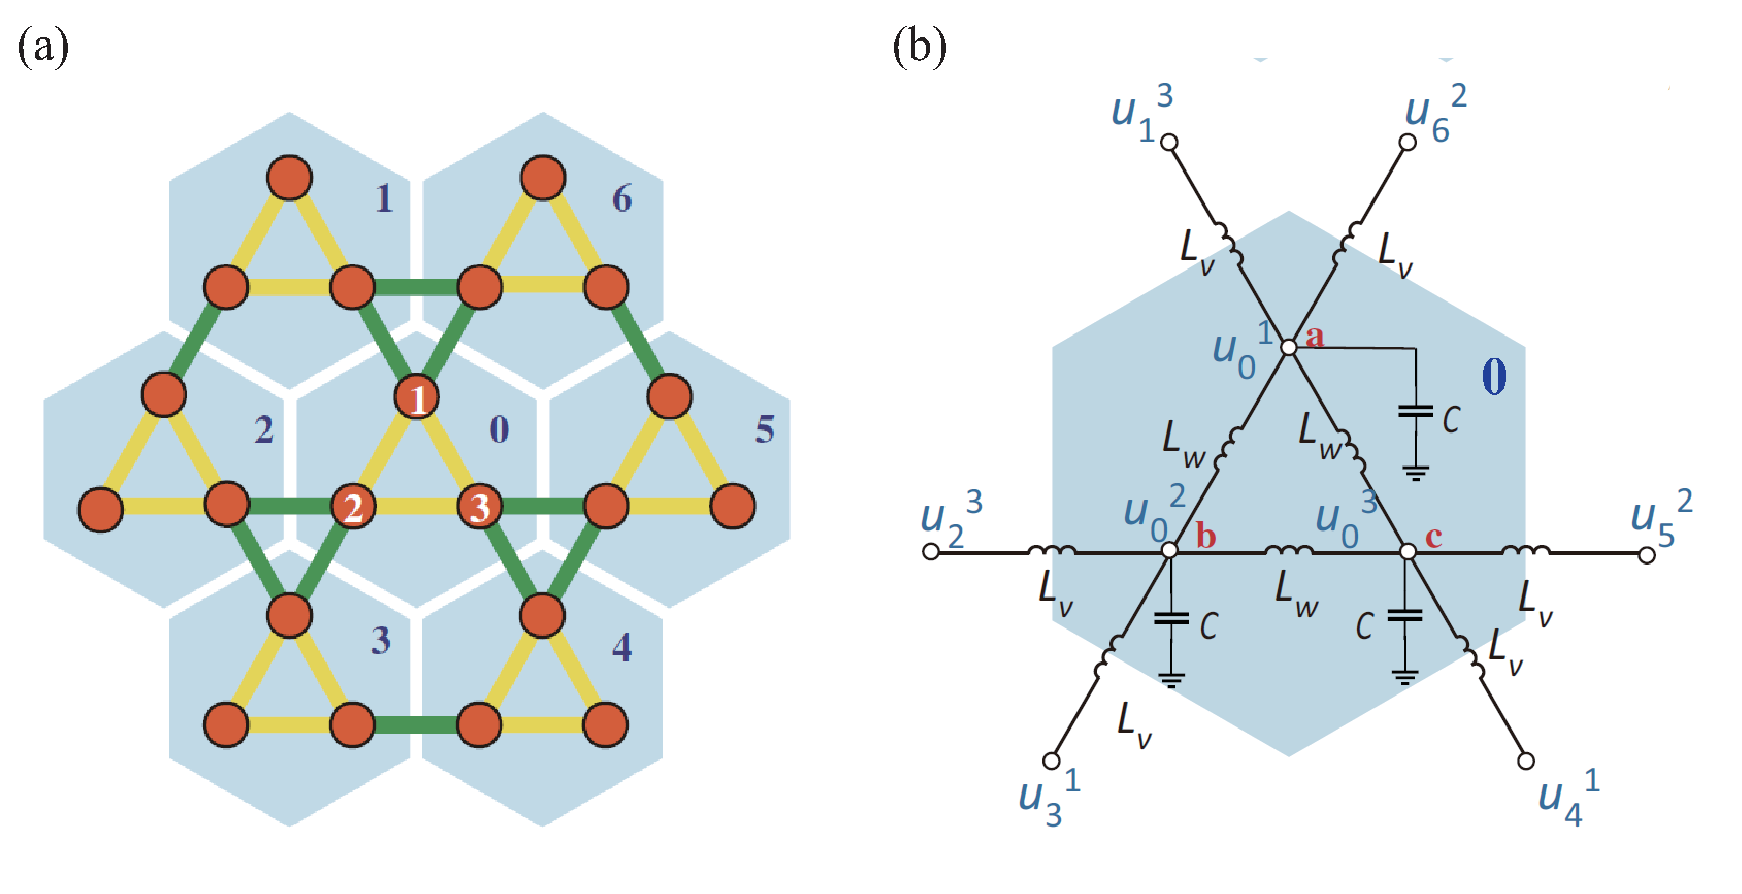
\includegraphics[width=1\textwidth]{images/fig3-2.eps} 
  \caption{Kagome声学系统体晶格的等效电路:
  (a)元胞Kagome晶格结构,其中晶格0居中,周围相邻的晶格分别编号为1到6。(b)晶格0的等效电路图。
  }
  \label{fig_3_2}
\end{figure}

如上一节所述,电子系统和声学系统有着相似性,我们可以构造声学腔管结构来类别电子Kagome晶格,也可以通过直觉调控其胞间和胞内的相互作用。在本节中,从声电类比方法出发,我们在亚波长尺度下从传统声学的角度严格推导出具有二维周期排列Kagome晶格的声共振系统的哈密顿量,从而揭示理论模型中的胞内或胞间跳跃与实际物理系统中的声学参数之间的联系。对于有限大结构,由于体,边,角上晶格的相邻晶格数量不同,我们也分别作了讨论。

首先,我们可以通过声学-电学类比来定义声学系统的 lumped 参数模型。如图\ref{fig_3_2}(a)所示,对于在周期结构中的晶格0而言,其周围有六个最近邻晶格,编号为1到6。单个晶格0的等效电路图如图\ref{fig_3_2}所示。在该电路模型中,腔体被表示为电容 \( C \),波导被表示为电感 \( L_v \) 和 \( L_w \)。具体公式如下:
\begin{equation} \label{eq3-1}
  C = \frac{V}{\rho c^2},
\end{equation}
\begin{equation} \label{eq3-2}
  L_v = \frac{\rho (l_v + 1.7r_v)}{\pi r_v^2}, \quad L_w = \frac{\rho (l_w + 1.7r_w)}{\pi r_w^2},
\end{equation}
其中,\( V \) 是腔体的体积,\( \rho \) 是空气的密度,\( c \) 是声速,\( r_v \) 和 \( r_w \) 分别是波导的半径,\( l_v \) 和 \( l_w \) 是它们的长度。

通过应用基尔霍夫电流定律,我们可以得到了描述声学波动的方程。对于周期性结构,腔体的声压在每个晶格点处满足如下方程:
\begin{subequations}\label{eq3-3}
  \begin{align}
  -(2w + 2v)u_{1}^{0} + wu_{2}^{0} + wu_{3}^{0} + vu_{2}^{6} + vu_{3}^{1} &= \omega^{2}u_{1}^{0}\label{eq:sub1}\\
  -(2w + 2v)u_{2}^{0} + wu_{3}^{0} + wu_{1}^{0} + vu_{3}^{2} + vu_{1}^{3} &= \omega^{2}u_{2}^{0}\label{eq:sub2}\\
  -(2w + 2v)u_{3}^{0} + wu_{1}^{0} + wu_{2}^{0} + vu_{1}^{4} + vu_{2}^{5} &= \omega^{2}u_{3}^{0}\label{eq:sub3}
  \end{align}
\end{subequations}
其中,$u_m^n$表示第$m$个晶格的第$n$个空腔中的声压,且$v = -1/L_vC$,$w = -1/L_wC$。对于一个周期性结构,它保证了$u_m^n$可以被描述为布洛赫波函数,方程(3)可以重写为矢量形式:
\begin{equation}\label{eq3-4}
  \mathcal{H}_{0}\mathbf{u} = \omega^{2}\mathbf{u},
\end{equation}
其中,$\mathbf{u} = [u_0^1\ u_0^2\ u_0^3]^{\mathrm{T}}$,并且$\mathcal{H}_{0}$可以表示为:
\begin{equation}\label{eq3-5}
  \mathcal{H}_{0}(\mathbf{k}) = 
  \begin{bmatrix}
  -2w - 2v & w + ve^{j\mathbf{k}\cdot(\mathbf{a}_{1}+\mathbf{a}_{2})} & w + ve^{j\mathbf{k}\cdot\mathbf{a}_{1}} \\
  w + ve^{-j\mathbf{k}\cdot(\mathbf{a}_{1}+\mathbf{a}_{2})} & -2w - 2v & w + ve^{-j\mathbf{k}\cdot\mathbf{a}_{2}} \\
  w + ve^{-j\mathbf{k}\cdot\mathbf{a}_{1}} & w + ve^{j\mathbf{k}\cdot\mathbf{a}_{2}} & -2w - 2v
  \end{bmatrix}
\end{equation}
其中,$\mathbf{k}$是布洛赫波矢,$\mathbf{a}_{1}$、$\mathbf{a}_{2}$表示晶格常数。显然可以看出,求解周期结构的共振频率及其相应的特征模式可归结于求解$\mathcal{H}_{0}$的本征值问题,这与电子系统的哈密顿量相对应,$w$和$v$对应于Kagome晶格的胞内跳跃和胞间跳跃。我们把$\mathcal{H}_{0}$称为无限大周期排列的Kagome结构的声学哈密顿量。

\begin{figure}[h!]
  \centering
  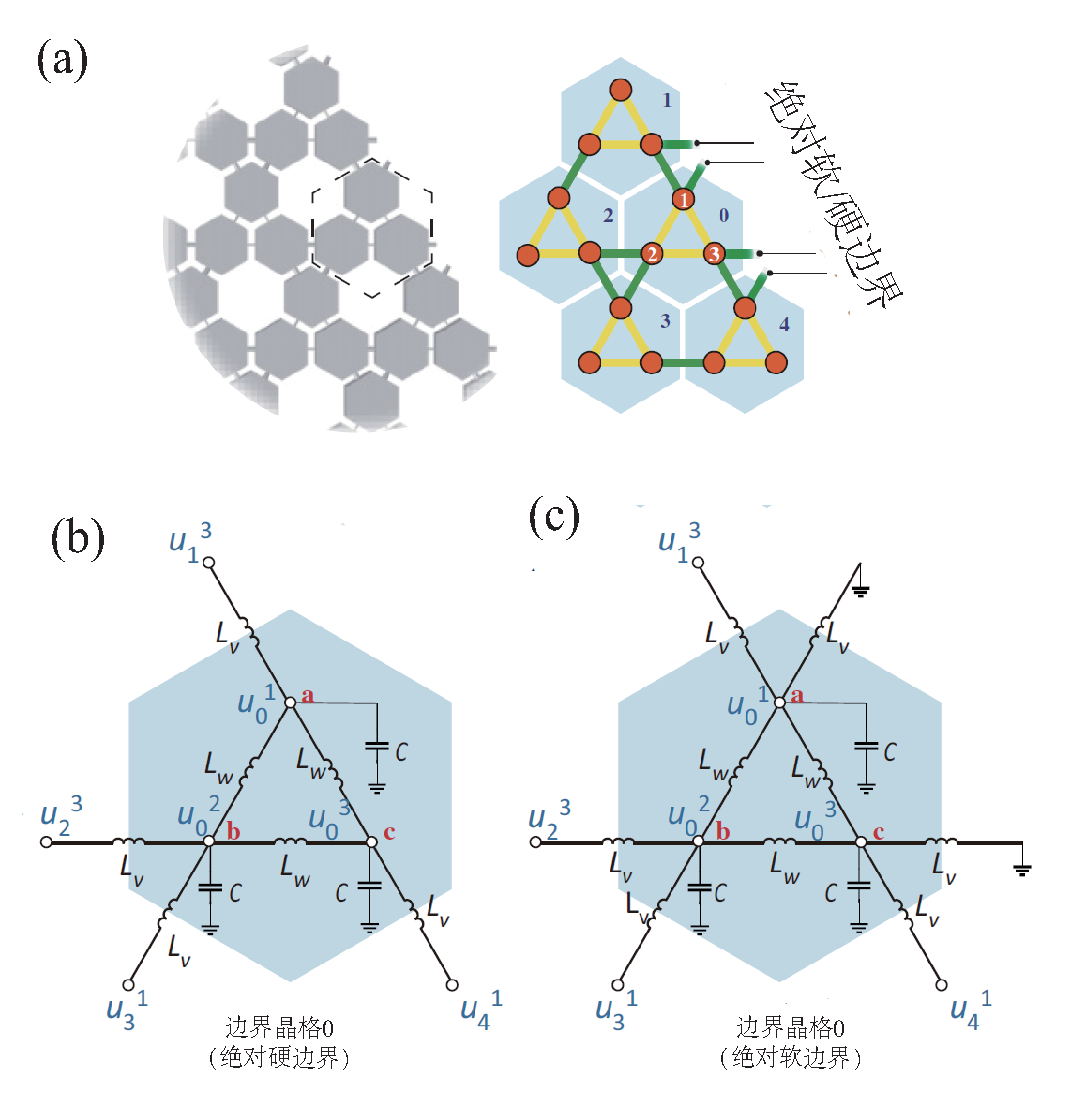
\includegraphics[width=1\textwidth]{images/fig3-3.eps} 
  \caption{Kagome声学系统边界上晶格的等效电路:
  (a)边界上Kagome晶格结构,其中晶格0为边上晶格,周围相邻的晶格分别编号为1到4。(b)绝对硬边界时晶格0的等效电路图。(b)绝对软边界时晶格0的等效电路图。
  }
  \label{fig_3_3}
\end{figure}

我们注意到,对于周期系统,该结构相应哈密顿量的对角项(式\ref{eq3-5})是相同的。然而,若考虑有限大系统的边界,由于边、角晶格相邻晶格的数目体晶格相邻晶格数目不同,这会导致哈密顿量的对角项。有限结构哈密顿量中对角项的差异会对拓扑性质产生巨大影响,这是由于广义手征对称性的差异所致,而广义手征对称性保护着拓扑态。我们以边界晶格为例说明这种有限大系统边界上哈密顿量随边界条件的改变,如图\ref{fig_3_3}所示,我们假设在有限结构的边缘存在一个晶格0。与图\ref{fig_3_2}(a)相比,图\ref{fig_3_3}(a)中的相邻晶格5和6被与之相连的最外层管道的硬边界或软边界所取代。在集总电路模型中,硬边界相当于断路情况,而软边界相当于接地,分别如图\ref{fig_3_3}(b)和图\ref{fig_3_3}(c)所示。相应地,对于硬边界情况,边缘晶格的方程可如下获得:
\begin{subequations}\label{eq3-6}
  \begin{align}
  -(2w + v)u_{0}^{1} + wu_{0}^{2} + wu_{0}^{3} + vu_{1}^{3} &= \omega^{2}u_{0}^{1}, \\
  -(2w + 2v)u_{0}^{2} + wu_{0}^{3} + wu_{0}^{1} + vu_{2}^{3} + vu_{3}^{1} &= \omega^{2}u_{0}^{2}, \\
  -(2w + v)u_{0}^{3} + wu_{0}^{1} + wu_{0}^{2} + vu_{4}^{1} &= \omega^{2}u_{0}^{3}, \
  \end{align}
\end{subequations}
而软边界情况的公式为:
\begin{subequations}\label{eq3-7}
  \begin{align}
  -(2w + 2v)u_{0}^{1} + wu_{0}^{2} + wu_{0}^{3} + vu_{1}^{3} &= \omega^{2}u_{0}^{1}, \\
  -(2w + 2v)u_{0}^{2} + wu_{0}^{3} + wu_{0}^{1} + vu_{2}^{3} + vu_{3}^{1} &= \omega^{2}u_{0}^{2}, \\
  -(2w + 2v)u_{0}^{3} + wu_{0}^{1} + wu_{0}^{2} + vu_{4}^{1} &= \omega^{2}u_{0}^{3}. 
  \end{align}
\end{subequations}
将方程\ref{eq3-6}与方程\ref{eq3-7}进行比较,可以明显看出边界条件的影响恰好反映在哈密顿量对角项的差异上。总体而言,软边界使得所有晶格(包括体晶格和边界晶格)的对角项都等于$-(2w + 2v)$。从这个角度来看,应用绝对软边界的有限大声学系统可以被视为是更接近电子系统的类比。

\section{Kagome晶格体能带与拓扑相变}

\begin{figure}[h!]
  \centering
  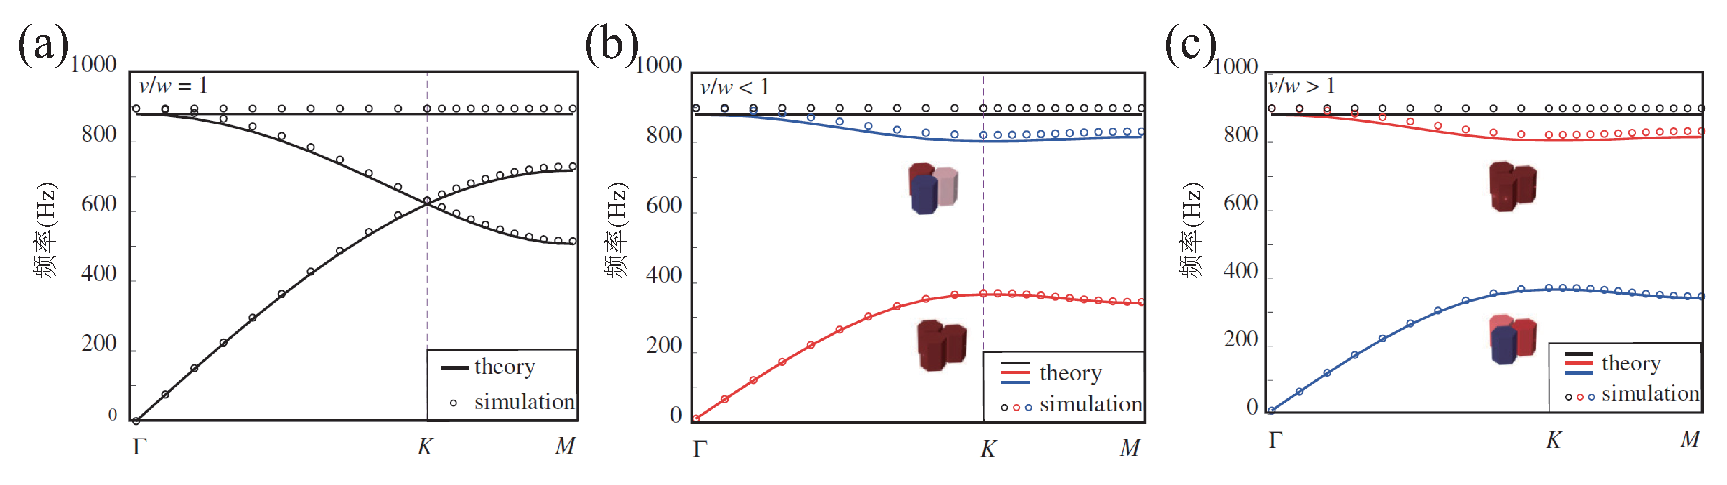
\includegraphics[width=1\textwidth]{images/fig3-4.eps} 
  \caption{Kagome声学系统的体能带:
  (a)$w=v$(b)绝对硬边界时晶格0的等效电路图。(b)绝对软边界时晶格0的等效电路图。
  }
  \label{fig_3_4}
\end{figure}

上一节中,我们推导了这种腔管结构的声学方程。接下来,我们研究这种晶格周期排列时的拓扑性质。在图\ref{fig_3_4}中,谐振器的边长和高度分别为$d = 10$(mm)和$h = 25$(mm)。波导管的长度为$l_w = l_v = 2.5$(mm),$V$是腔体的体积。空气的质量密度和相应的声速分别定义为$\rho = 1.23$(kg/m³)和$c = 343$(m/s)。一般来说,带反转发生在胞间跳跃的变化处,此模型中的胞间跳跃和胞内跳跃由胞间管半径$r_w$和胞内管半径$r_v$分别确定。

使用COMSOL Multiphysics进行模拟,图\ref{fig_3_4}描绘了当$r_w = r_v = 0.55$(mm),$r_w = 0.75$(mm)且$r_v = 0.3$(mm),$r_v = 0.3$(mm)且$r_v = 0.75$(mm)时的能带结构。由$v = -1/L_vC$,$w = -1/L_wC$,这三种情况分别对应$v/w=1$,$v/w<1$和$v/w>1$。三个图中的平带来自于相消干涉,这导致了紧致局域态,而另外两条能带反映了拓扑性质。可以明显看出,当$r_w = r_v$时,存在一个受对称性保护的狄拉克锥,这表明拓扑相变的临界点。对于$C_3$对称晶格,体极化$p_l$定义为:
\begin{equation} \label{eq3-8}
  e^{-i\pi p_l} = \prod_{n \in \text{occ}} \frac{\theta_n(\mathbf{K})}{\theta_n(\Gamma)},
\end{equation}
其中$\theta_n(\mathbf{k}) = (u_n(\mathbf{k})|R_{3}|u_n(\mathbf{k}))$是通过将三重对称算子$R_3$(旋转$2\pi/3$)应用于晶格高对称点处相应的布洛赫波函数$u_n(\mathbf{k})$计算得到的,“occ”表示占据带。由于只有一个能带位于带隙下方,体极化可表示为:
\begin{equation} \label{eq3-9}
  (p_1,p_2) = 
  \begin{cases}
  (-1/3,-1/3), & w < v \\
  (0,0), & w > v
  \end{cases}
\end{equation}
因此,当$w < v$时的非零极化表明了能带的非平凡拓扑相,而当$w > v$时则表示平凡相。由于所有原子被认为是相同的,边界诱导的填充异常预计将沿着非平凡体极化情况被诱导,这由拓扑边缘态的存在表示,此时边界是开放的。同时,当所有原子在热力学极限下相同时,也可以诱导出由低维拓扑角态表征的角诱导填充异常。

到目前为止,我们讨论的是所有原子在热力学极限下相同的情况。然而,在下一节中,我们将展示当涉及到封闭经典系统时,系统的onsite能量(体现为哈密顿量的对角项)总是受到边界的影响。

\section{Kagome晶格的边界态和角态}

\section{边界条件对拓扑态的影响}